%%%%%%%%%%%%%%%%%%%%%%%%%%%%%%%%%%%%%%
%%  
%% Chapter 1: Introduction to heterogeneous computing
%%
%%%%%%%%%%%%%%%%%%%%%%%%%%%%%%%%%%%%%%

\def\ArtDir{01.HeteroComp/figures}%

\chapter{Heterogeneity and the future of computing}
\label{chapter:heterogeneity}

How do you summarize over 40 years of computing history in a couple pages?   
Think of a pendulum swinging from one extreme to another.  The pendulum spends very little time at
the low-point where forces are balanced.  In fact, that point is precisely where the pendulum is
moving the fastest and those trying to follow the motion must struggle the most  to keep up.

This mental model is a good way to think about the history of computing.  We could start with the
works of Babbage or much later with Turing, but for the sake of brevity, let's start with the era of computing
that emerged with the microprocessor.  In those days (the late 1970s and early '80s) a programmer
needed to understand the low level details of the system.  A professional programmer as a matter
of their normal work-day wrote in low level languages regularly dropping down to assembly code 
when needed.   Programming was a matter of understanding hardware bottlenecks and then working at the lowest 
level to knock them back to get these computers (primitive by today's standards) to do what was needed.

As the '80s progressed and the full force of Moore's Law kicked in, the game changed.   With
microprocessor performance doubling every year, a programmer was actually punished for 
working hard to optimize code for a particular system.  The pendulum had swung from
a world where the programmer was almost a hardware engineer to the opposite.  The ability to 
add new features instead became the focus.  Productivity and portability where the driving concerns and
programmers came to think of themselves as software engineers working to make ever more
complex programs correct and full-featured.

In the early '90s with the introduction of out-of-order execution for a microprocessor's instructions, the 
pendulum had reached an extremity where the need to write assembly code fell to the side.  Object-oriented
programming and other high level concepts were the talk of the town for software engineers.  Performance was
truly the job of the hardware and we all rode the coattails of Moore's Law into a bright future of
ubiquitous computers filling every facet of our lives.

Pendulums, however, keep moving.  In the early 2000s the ability to manage static effects such as electrical
leakage came to dominate.   Power densities made cooling a major problem.  Manufacturing the microprocessors was harder. Moore's Law was 
still with us, but it could no longer be used to double performance every couple years.
As Herb Sutter famously observed, ``the free lunch'' for software engineers was over. 

This is all ancient history at this point.  Multicore chips emerged.  Core counts were small, cache hierarchies were 
simple, and DRAM cost models were relatively flat.   People had to write multithreaded programs.   While OpenMP
was born to program supercomputers in the years before multicore chips,
the transition to ubiquitous multicore chips pulled OpenMP into the mainstream.  This was great for 
old-timers who still remembered the old-days of hardware-centered programming (that is, the sort of people 
who created OpenMP in the first place). For the masses of programmers, however, these were dark days.
Understanding hardware and utilizing that deep understanding became a requirement once again to write performant code.

We hoped the pendulum would swung through the low point in its journey and that language/compiler technology
would take us back to a time when programmers didn't have to spend their days coding to low level features of the
hardware.  We were wrong.  The pendulum swing into hardware-aware programming was just getting started.
First there were the many-core chips with non-uniform memory cost models that required programmers to understand
where their threads executed and how they lined up with memory.  Then Chaos struck the life of programmers again with
the advent of heterogeneous computing.

The idea is simple, though the software response is anything but simple.  Hardware specialized to a specific task is
more power-efficient than general purpose hardware.   If your application does computations that look like a graphics pipeline, 
use a GPU: a processor specialized for graphics processing.  If you are operating over arrays of high-dimensionality containing dense blocks
(a pattern commonly found in Deep Learning applications), use a Tensor Processor Unit.  If
you are coordinating execution over a wide range of storage, networking, and computational elements, use an infrastructure
processing unit. A system composed of heterogeneous hardware elements is a system that for a fixed amount of power runs faster.
This is called \emph{heterogeneous computing}.   It's not about moving the work from a CPU onto a GPU, and then once there 
keeping the work there (something we call \emph{offloading}).   It's the old game of organizing a computation 
so the ``whole is greater than the sum of the parts'' by matching each part of your program to the hardware for which it is best suited.

And this is where the pendulum sits today.   Programmers need to understand a great deal about the hardware.  Programmers need to 
know which classes of algorithms map to which types of hardware.  Programmers need to understand how to target one block of 
code to a throughput optimized device (e.g. a GPU) while another block of code asynchronously runs on another device
that may be latency optimized (e.g. a CPU).  The pendulum will swing back.  Some day, the tools programmers use will 
hide those details from programmers.   That day, however, is not today.   And let's face it, when the pendulum swings to the
blissful extreme of programming productivity where hardware is hidden behind layers of abstraction, we know it will someday
swing back again.  That's just how computing seems to work.

In this book, we will explore heterogeneous computing and how your can write programs that exploit heterogeneity 
using OpenMP.  We are in a world where you have to understand hardware and how software maps onto it.   You can 
complain about that state of affairs or accept it and figure out how to move forward.  OpenMP is an explicit API.  You 
tell the compiler what to do through directives and a supporting API, and it does what you say.    In this book we will
explain how all of that works and, in the process, tell you about the key design patterns used in heterogeneous computing.

Our journey begins with this chapter.  We set the stage with a brief description of the hardware we use when
running programs written with OpenMP.   Even experienced parallel programmers with detailed knowledge of
parallel hardware should skim this chapter to make sure we are on the same page concerning the jargon used
for describing hardware.

\section{The basic building blocks of modern computing}

Computer architecture is a fascinating field. If you want to master it, read the
famous text book we all learned it from (Hennessy and Patterson).  For our purposes
here, we will simplify the problem by thinking in terms of three basic processor building blocks.

\begin{itemize}
\item  the CPU
\item  the SIMD Vector Unit
\item  the GPU
\end{itemize}

We skip many important developments in computer architecture with this oversimplification, but 
it turns out that most of what you need to know as an application programmer working in 
heterogeneous computing can be addressed in terms of these three basic building blocks.
We will consider each in turn.

\subsection{The CPU}

A CPU is a device optimized for latency sensitive computing.  You click your mouse and you expect something to happen
immediately.  Of course there is always a delay which is a span of time we call the ``latency''.  As long as this
latency is small on a human time scale (less than 50 microseconds), the user feels the computer is delivering results
instantaneously and  all is well.  

Low latency computing is difficult.  The time to reference an item in memory (DRAM) is around 100 nanoseconds.  This latency
seems quite small, but not when you consider that a modern CPU completes basic arithmetic operations in well
under a nanosecond.  With orders of magnitude differences between the speeds of the CPU cores and the performance
of memory, a CPU keeps high speed blocks of memory (SRAM) close to the cores.  These are organized as a 
cache hierarchy to maintain a window into DRAM memory.  As long as the items needed from memory 
reside in cache, all is well and low latencies are provided.  

We show a typical server in figure~\ref{figure:CPU} with a common configuration of CPUs.   
We show this figure to drive home the fact that the cache hierarchy is complicated.  The design
of the CPU is optimized around managing memory to deliver low latencies.   Each core may
support a number of hardware threads (in the figure there are two: $HT_0$ and $HT_1$).  By switching between the two threads
while the core executes, the various arithmetic logic units ($ALU$) are more likely to be fully consumed.
On each core is a pair of L1 caches, one for instructions and one for
data.  They share a unified L2 cache.   Those caches keep data close to the CPU cores to hide the latency
of access to main-memory (through the pair of DDR memory controllers on each CPU).  The speed differences
between memory and the cores is so great, however, that we often find another level of cache.  This is the L3 
cache broken down into blocks and spread out around the chip.   And that's not all.  There are cache coherency
protocols that run between the pair of CPUs (through the QPI ports, a bus which connects the two sockets) 
so our windows into memory (dynamic Random Access memory or \emph{DRAM}) are
consistent between the two CPUs.  These two CPUs and all of their cores share a common view of memory. 
Ideally this view is the same from any one core to any location in memory. This arrangement is often 
called a Symmetric Multiprocessor (SMP).   Note, however, that SMP is an idealization and the fact of the matter
is that due to multiple memory controllers (DDR) and the cache hierarchy, the cost function for a memory-access is
anything but uniform and therefore the system in figure~\ref{figure:CPU} is a Non-Uniform Memory Architecture (NUMA).
We won't explore NUMA issues in this book\footnote{The concept of SMP as an idealization. The implications
for NUMA in the context of OpenMP is discussed at length in the book \emph{Using OpenMP: the Next Step}, published by MIT Press.}.

\begin{figure}[t]
\centerline{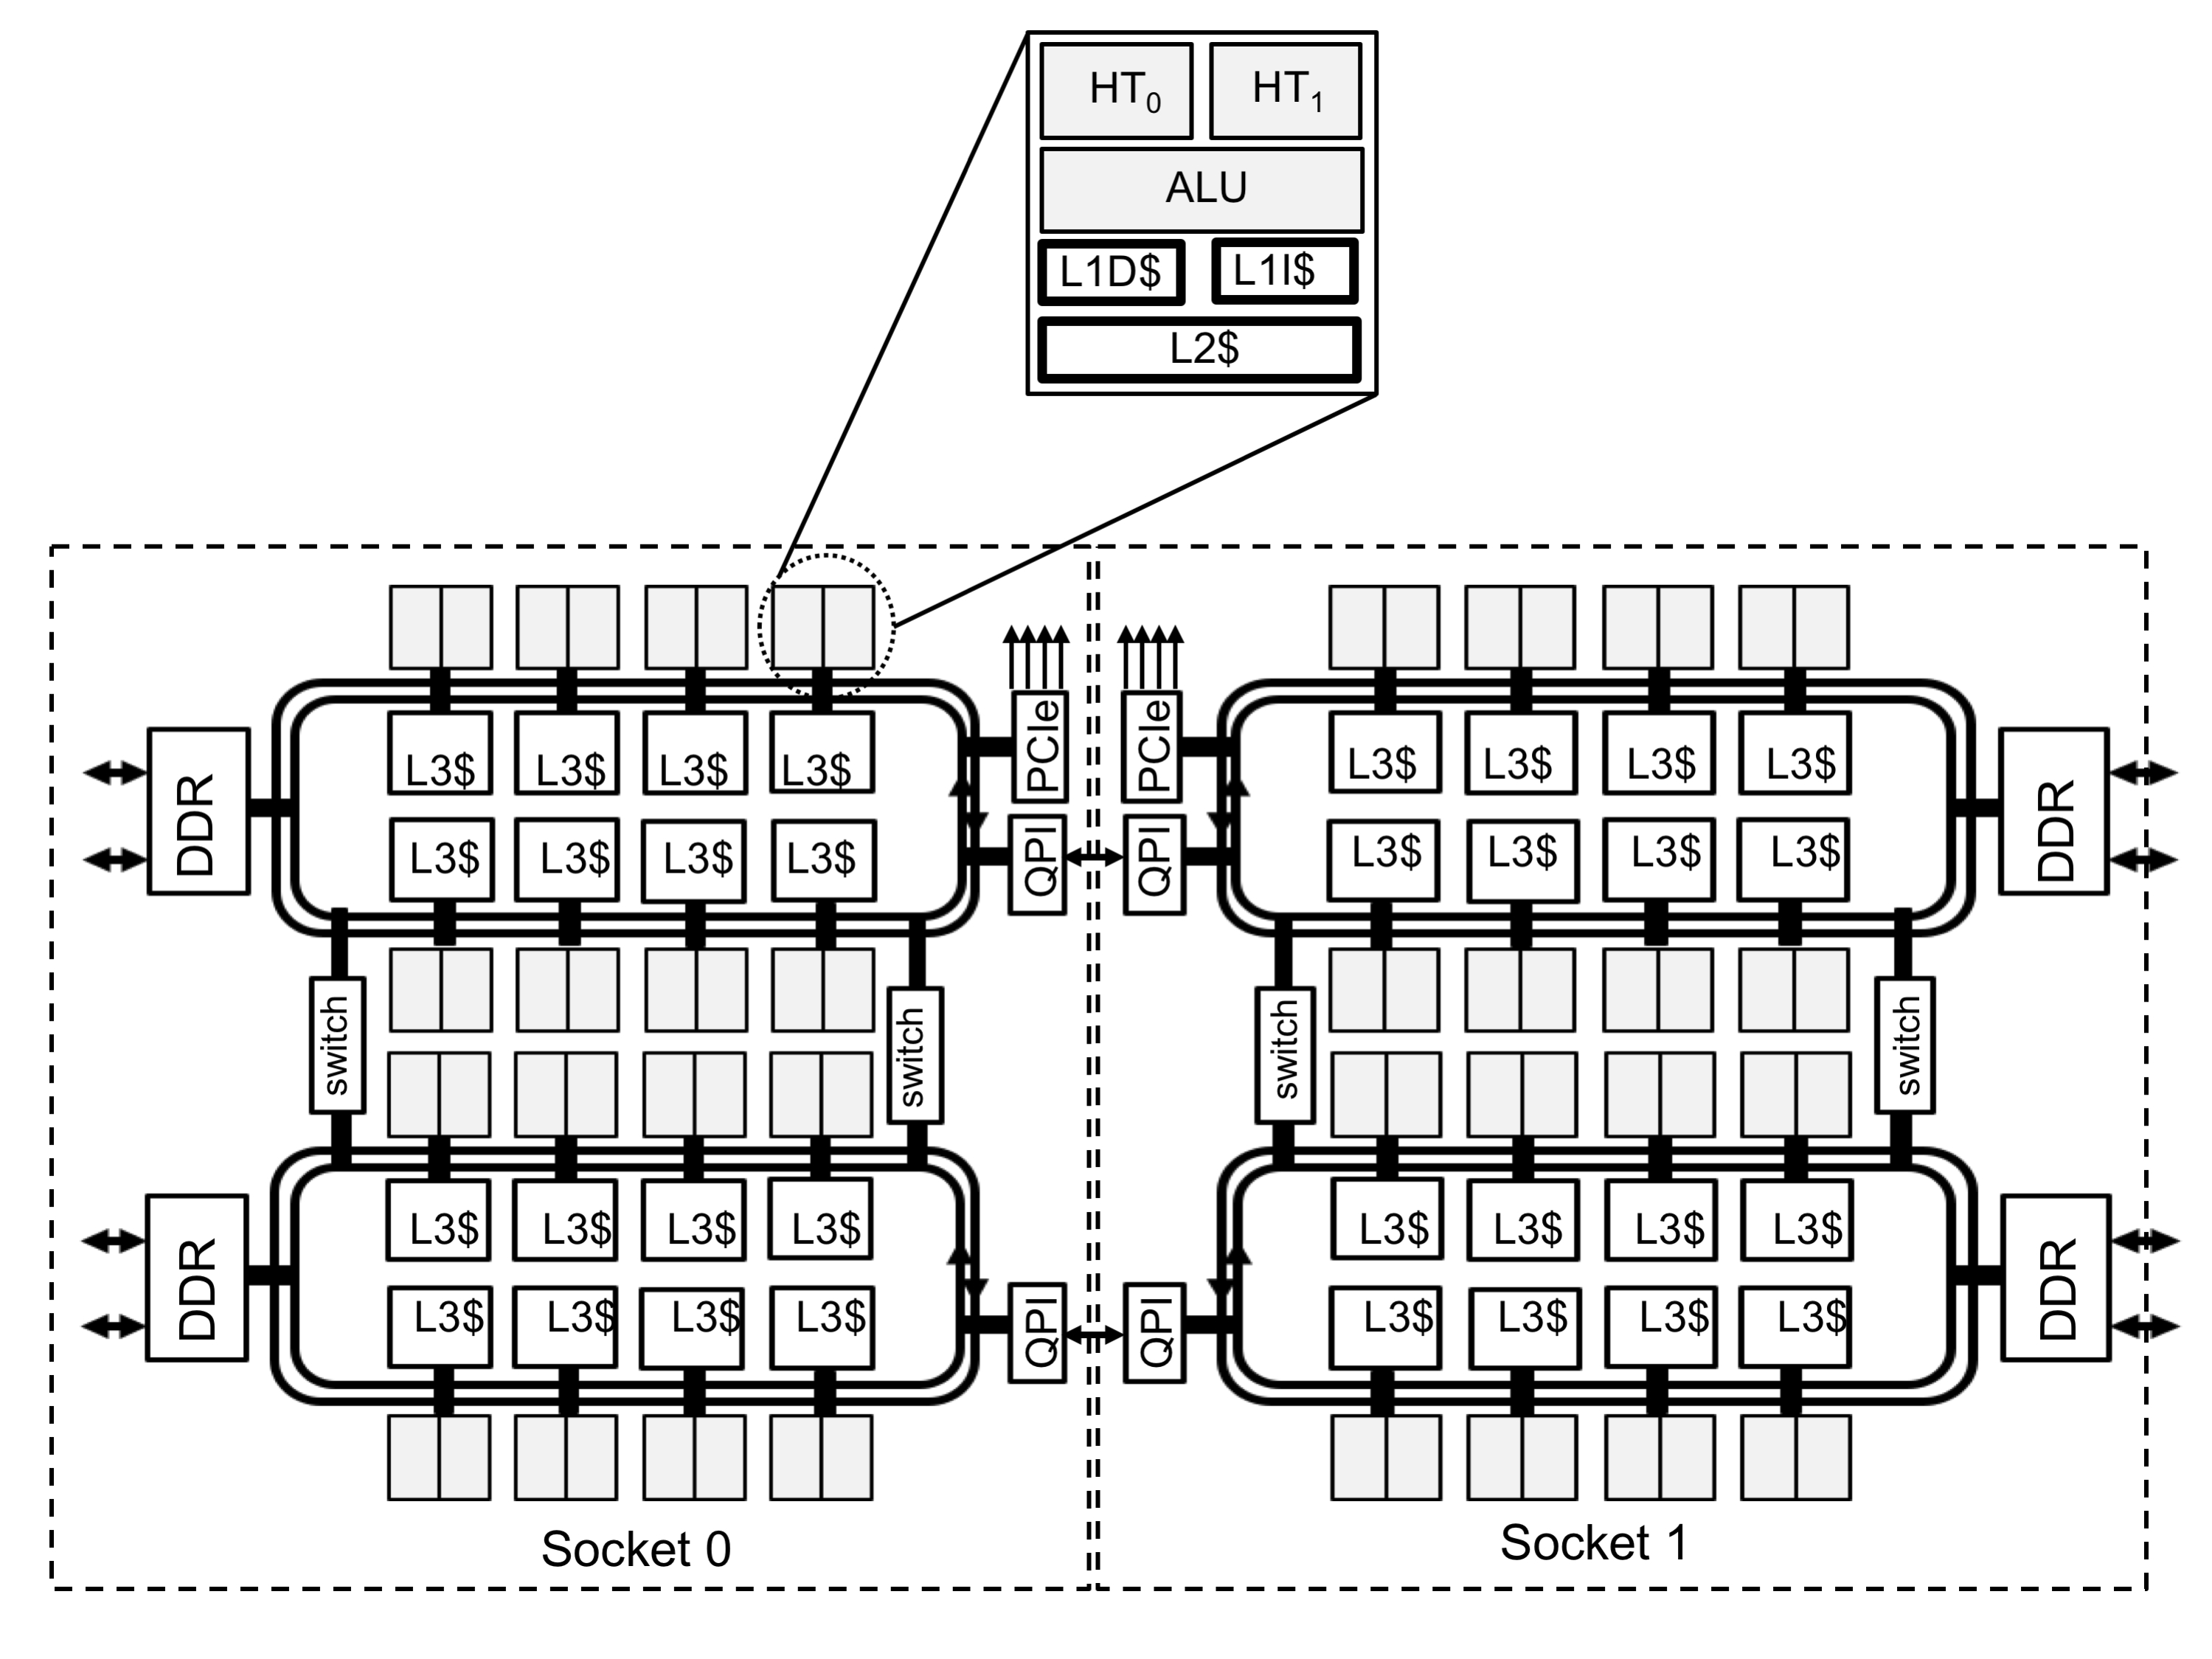
\includegraphics[width=400pt]{\ArtDir/CPU}}
\caption{A block diagram of a typical server consisting of two sockets with each socket holding a CPU. Each
CPU has 16 CPUs the details of which are shown for one core.}
\label{figure:CPU}
\end{figure}

The CPU memory hierarchy is complicated and consumes a great deal of design-effort and chip area.  
When data access patterns are regular and the data needed by a core is likely to be in cache, all is well and 
the latencies observed by the human using the chip are low.  However, if the data needed by a program is
not in the cache, latencies fall off and the chip can't keep up with the demands of interactive computing.

One solution to this problem is for the CPU to exploit the concurrency in the workflows run on the system.
The term \emph{concurrency}\index{Concurrency} is seriously abused in computer science literature so we will
take the time to define it here.   Consider the work carried out in a program.   We can break this work into 
distinct units of work.  When multiple units of work (usually called a ``thread'' on a CPU) are 
available to be scheduled for execution and they are unordered with respect to each other, we say those threads are concurrent.  
There are many ways an Operating System can schedule concurrent threads.  
The most common approach is called \emph{time-slicing}\index{time-slicing} where the OS gives
each thread a small block of time to execute moving quickly from one thread to the next.  
If each thread is given an equal chance
to become active and make forward progress through its work, we say the scheduling is \emph{fair}.  With fair scheduling\index{Fair scheduling}
and concurrent threads, the system swaps from one thread to the next so it appears to the user that all the threads
are making forward progress at the same time (assuming they are not blocked and waiting on a resource).   This, in essence, makes the
software expressed in terms of concurrent threads appear more responsive and therefore supports interactive use.

All modern operating systems and most commercial-grade applications running on CPUs utilize multiple threads to
exploit concurrency and support low latency, interactive computing.  When there are large numbers
of threads to schedule across a CPU, we can increase the speed at which the threads complete their work by adding multiple 
cores, supplying the threads with more physical hardware resources.  When a workflow has concurrency (to support multiple threads) and we exploit that concurrency by running on 
multiple cores, we say that that workflow is running ``in parallel''.  

Concurrency and Parallelism\index{Parallelism} are closely related but 
different.  Concurrency\index{Concurrency} deals with unordered units-of-work available for execution on a system.  Parallelism takes those  
units-of-work and runs them at the same time.  Concurrency is used even on one core to support 
responsive computing, so work can proceed from one unit-of-work while another is blocked waiting on some resource (such as 
memory).  Parallelism is only at play when multiple units-of-work are \emph{actually} making progress at the same time.  We will have 
much more to say about concurrency later when we talk about synchronization between units-of-work on a GPU.

\subsection{The SIMD Vector Unit}

We can think of high performance computing applications as programs where performance is a feature.
The goal is to a fixed body or work done in less time or conversely, to complete more work in a fixed unit of time.
In both cases, a key ingredient is to complete the rate at which operations complete.   

A CPU does this with multithreading; that is, concurrent threads running in parallel across a collection of cores. 
Another approach is to use parallelism that is ``in the data'' where a stream of instructions are applied in
parallel to a collection of data elements.  We call this 
SIMD\index{SIMD} or ``Single Instruction Multiple Data''\index{Single Instruction Multiple Data} parallelism.

Problems that can exploit SIMD parallelism occur when they can be expressed as a sequence of
operations that operate on dese arrays of data.   These problems are common enough that SIMD units optimized
for vectors have become one of the standard building blocks of parallel architectures.  To see
how they are used, it helps to consider an example.  Consider the loop in figure~\ref{code:vaddLoop}.  
We add vector $A$ to vector $B$ to produce the result $C$.   


\begin{CodeExample}%
{\textbf{Vector Add program} --\small This program will add two vectors of length $N$
to produce a third vector.
}%
{code:vaddLoop}
\begin{lstlisting}
#define N 4000;

int main()
{

   double A[N], B[N], C[N];
     
   init(A,B,C); // initialize arrays ... code not shown
   
   for (int i = 0; i < N; i++) {
      C[i] = A[i] + B[i];
   }
}	  
\end{lstlisting}
\end{CodeExample}


A computational element called a \emph{vector unit}
will use SIMD parallelism to execute blocks of instructions between elements of these three arrays.  
Let's consider a case where our vector unit is 256 bits
wide so we can process four 64-bit floating point operations in instruction of the vector unit.  You write
vector code in two distinct phases. First, you transform the code so the loop matches the one you'll
need for the vectorized code.   In this case, tht means we need to 
modify the loop so the loop body carries out four additions of the vector elements per loop iteration.
This is called unrolling a loop.  We show our loop unrolled by four in figure~\ref{code:vaddUnroll}.  

\begin{CodeExample}%
{\textbf{Vector Add program unrolled} --\small We unroll our vector addition loop by four meaning
the loop body acts on four elements of the data (4 64 bit numbers for a 256 bit wide vector unit).   For 
simplicity, we require that N can be evenly divided by 4.
}%
{code:vaddUnroll}
\begin{lstlisting}
#include <assert.h>
#define N 4000;

int main()
{
   double A[N], B[N], C[N];
   
   init(A,B,C); // initialize arrays ... code not shown
   
   assert(N%4==0);

   for (int i = 0;i < N4; i=i+4) {
      C[i]     = A[i]     + B[i];
      C[i+1] = A[i+1] + B[i+1];
      C[i+2] = A[i+2] + B[i+2];
      C[i+3] = A[i+3] + B[i+3];   
   }
}	  
\end{lstlisting}
\end{CodeExample}

In the second phase of our vectorization process, we replace the operations over scalar values with vector instructions.
We will use the well-known Advanced Vector Extensions (AVX) introduced in 2008. The resulting vector code is
shown in figure~\ref{code:vaddVec}.  In this code, we use the following AVX instructions.  
\begin{itemize}
\item \Code{ __m256d}: The type for the 256 bit wide vector register to hold (in our case) four 64-bit floating point numbers.
\item \Code{_mm256_loadu_pd()}:  loads 4 doubles (pd or ``packed double'') from an address that may not be aligned on a 32 byte boundary.
\item \Code{_mm256_storeu_pd()}:  stores 4 doubles to an address that may not be aligned on a 32 byte boundary.
\item \Code{_mm256_add_pd()}: adds  two vector registers holding double precision floating point numbers to return 
their sum in another vector register.
\end{itemize}
We would compile this code as \Code{gcc -mavx}.  The above operations assume the data is unaligned.  
For best efficiency, the arrays \Code{A, B, C} should be 
aligned to a 32 byte boundary.  We can do this by allocating the memory for these arrays using the following statement.
\begin{verbatim}
double *A = (double *)aligned_alloc(32,N*sizeof(double));
\end{verbatim}
When the workflow in a program maps onto a vector unit, the performance 
benefits are substantial.

\begin{CodeExample}%
{\textbf{Vector Add program with vector intrinsics} --\small We use vector intrinsics to compute 
4 additions in parallel across the lanes of our SIMD vector unit. 
}%
{code:vaddVec}
\begin{lstlisting}
#include <assert.h>
#include <immintrin.h>
#define N 4000;

int main()
{
   double A[N], B[N], C[N];
   // 256 bit vector registers to be packed with double precision numbers
   __m256d Avec, Bvec, Cvec;    
     
   init(A,B,C); // initialize arrays ... code not shown
   
   assert(N\%4==0);

   for (int i=0; i<N; i=i+4){

       Avec = _mm256_loadu_pd(&A[i]);
       Bvec = _mm256_loadu_pd(&B[i]);
       Cvec = _mm256_add_pd(Avec,Bvec);
      _mm256_storeu_pd(&C[i],Cvec);
   }
 }
\end{lstlisting}
\end{CodeExample}



Most programmers, however, do not write vector code directly.  The compiler unrolls the loop, organizes the instructions for SIMD
execution, and replaces them with specialized vector instructions.  In an ideal world, that would be good enough. Indeed,
for a simple case such as vector addition, the compiler does quite well.  In practice, however, codes do not so directly map
onto vector instructions and the exploitation of the vector units are often quite poor.
To help the compiler with transformations needed to support vectorization (such as loop unrolling) OpenMP added
a SIMD construct and a collection of clauses\footnote{SIMD in the context of OpenMP is discussed at length in the book
\emph{Using OpenMP: the Next Step}, published by MIT Press.}.

Vector units for SIMD parallelism are rapidly evolving.  The widths of the vector units are commonly 256 on lower-end
CPUs and have climbed up to 512 or even 1024 for CPUs used in high-end servers.  There is no reason the concept must 
be restricted to one dimension vectors.   SIMD units for two dimension arrays have appeared on the market optimized
for the matrix-multiply operations common inside Deep Learning pipelines. 

Vector instructions operate on vector registers to operate on multiple data elements in parallel. There is a second (and equivalent)
way to think about vector instructions.   It's a perspective where you transpose your view and think in terms of scalar operations
happening on lanes of the vector unit, or the \emph{SIMD lanes}.   For example, the sequence over packed doubles
with 256 bit vector instructions:
\begin{verbatim}
   Cvec = _mm256_add_pd(Avec,Bvec);
   Dvec = _mm256_add_pd(Avec,Cvec);
   Fvec = _mm256_add_pd(Bvec,Dvec);
\end{verbatim}
can be considered as four SIMD lanes
\begin{verbatim}
   SIMD-Lane0:  C[0] = A[0] + B[0]; D[0] = A[0]+C[0]; F[0] = B[0] + D[0];
   SIMD-Lane1:  C[1] = A[1] + B[1]; D[1] = A[1]+C[1]; F[1] = B[1] + D[1];
   SIMD-Lane2:  C[2] = A[2] + B[2]; D[2] = A[2]+C[2]; F[2] = B[2] + D[2];
   SIMD-Lane3:  C[3] = A[3] + B[3]; D[3] = A[3]+C[3]; F[3] = B[3] + D[3];
\end{verbatim}
The computation is the same in both cases as far as the hardware in concerned.  Thinking in terms
of SIMD lanes, however, is a useful abstraction for programmers trying to understand their vector code,
especially for more complex streams of instructions.  In essence, the vector lanes act like scale processing 
elements execution in lockstep through the stream of instructions.   
   
   
\subsection{The GPU}

A program defines work to be carried out by a computer.  The work is divided into distinct units or ``work-items''.  A GPU
is a processor optimized for throughput, that is, the time needed to complete work on the full set of work-items.
The latency for any particular work-item may be highly variable and much longer than other items in the set.
The concurrency across the set of work-items, however, is utilized to execute them in parallel and complete the 
full set as quickly as possible.  We show a block diagram for a typical (and somewhat idealized) 
GPU in figure~\ref{figure:GPU}.

\begin{figure}[!htbp]
\centerline{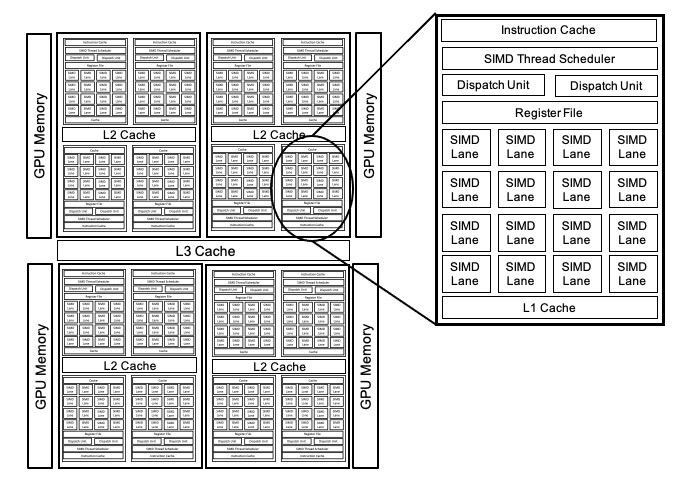
\includegraphics[width=400pt]{\ArtDir/GPU}}
\caption{A simplified block diagram of a typical GPU.  The computing within the GPU happens in the
SIMD lanes of a multithreaded SIMD Processor which in addition to the SIMD lanes often includes
load/store and special function units (not shown in this diagram).   The multithreaded SIMD processors
are organized hierarchically around caches and on-device GPU memory.}
\label{figure:GPU}
\end{figure}

GPUs for ``general purpose programming'' (GPGPU) are young compared to CPUs.  
While the terms used with CPUs are well established,
the terminology of GPUs varies widely between different GPU vendors and programming
languages.  To help pull the concepts together, we review the terminology from three
different sources in table~\ref{table:GPUjargon}: Hennessy and 
Patterson\footnote{Computer Architecture: A Quantitative Approach, Sixth Edition, 
John L. Hennessy and David A. Patterson, Morgan Kaufmann, 2019.}, Nvidia's CUDA, 
and OpenCL from the Khronos Group.

\begin{table}[!htbp]
\centering
\caption{\textbf{GPU Terminology: } 
-- \small
GPU Terminology Hennesy and Patterson, CUDA, and 
OpenCL.   The one uncertain match is the last row;
a sub-group usually corresponds to a warp, but a conforming implementation of OpenCL 
may use a subgroup to refer to smaller blocks of work-items that make up a warp.}
\label{table:GPUjargon}
\begin{tabular}{|l|l|l|}
\hline
\textbf{Hennessy and Patterson}  & \textbf{CUDA} & \textbf{OpenCL} \\
\hline
%============================================================
Multithreaded SIMD Processor    & Streaming multiprocessor & Compute Unit \\
\hline
SIMD Thead Scheduler               & Warp Scheduler                 & Work-group scheduler \\
\hline
SIMD Lane                                  & CUDA Core                        & Processing Element \\
\hline
GPU Memory                              & Global Memory                   & Global Memory \\
\hline
Private Memory                          & Local Memory                     & Private Memory \\
\hline
Local Memory                            & Shared Memory                   & Local Memory \\
\hline
Vectorizable Loop                       & Grid                                     & NDRange \\
\hline
Sequence of SIMD Lane operations & CUDA Thread                & work-item \\
\hline
A thread of SIMD instructions            & Warp                              & sub-group \\
\hline
\end{tabular}
\end{table}








I will talk about the history of the GPU.  How they started as an accelerator for graphics applications but over time
more and more programmable features were added to the GPU.  In 2006 with the introduction of CUDA and 
OpenCL just a couple years later, the GPU became a fully programmable device.   This is often called GPGU or
general purpose GPU programming.

The date 2006 is important.  While CPUs as microprocessors date back to1971 with the Intel 4004, fully
programmable GPUs are a much younger technology.  Hence, they are evolving rapidly.  Hence, we will describe them
at a high level sufficient to understand what you need to program them wtih OpenMP, we will not spend time with the low
level details of any particular GPU.   

I will then talk about the general organization of a GPU using my new figure.  I might add a table showing the NVIDIA/CUDA 
and OpenCL/Generic names.  In particular work-item vs. CUDA-thread, Compute-unit vs. Streamming multiprocessor, 
and PE vs CUDA-core.  I also need to talk about the host/device split and global vs. shared vs. private memory.

I want to talk about the core programming  model behind GPUs.  I'll show the standard loop vs. SIMIT for vector add.  I might
show the code for OpenCL and CUDA kernels in this case.  I'll talk about the index map, kernels, and kernel instances at each point
in the index map.


\subsection{Tom's text for The GPU section}

When discussing parallel programming models in general, is it sometimes important to distinguish between concurrent concepts in the programming model and parts of the hardware.
On CPUs for instance, parallel items called perhaps ``threads'' are assigned to run on physical parts of the CPU called perhaps ``cores''.
This correspondence is not necessarily unique, and parallelism expressed in the programming model may be assigned physical components of the processor in a number of ways.

OpenMP does not give sufficient terminology to name the underlying hardware of a given abstract device, and so to help throughout this book, we define an underlying target device using terminology borrowed from another open-standard programming model called OpenCL (from Khronos).
This is no criticism of OpenMP for it is typically an implementation detail on how the parallel concepts in OpenMP might correspond to physical, real-life hardware.
However in our situation, it is helpful to speak in terms regarding expressing parallelism in OpenMP differently to how that might correspond at run-time to the physical hardware.

A target device is constructed with a hierarchical structure of hardware.
The target device is built from a number of Compute Units (CUs)\index{Compute Unit}.
Each Compute Unit is formed from a number of Processing Elements (PEs)\index{Processing Element}.
The Processing Elements themselves are the hardware that can execute the program instructions, and are organised into Compute Units.
Processing Elements can operate independently but there is normally close ties with the other Processing Elements within the Compute Unit.
There is normally no (or little) interaction between Processing Elements in different Compute Units.
In particular, Processing Elements are not allowed to communicate with each other unless they reside in the same Compute Unit.

Each Processing Element may be able to execute vector (SIMD) instructions\index{SIMD}, and so might contain the requisite hardware for this.
The number of data elements the SIMD instructions process is called the width.
We call the location of each data item within the instruction a SIMD lane\index{SIMD lane}.

This three level hierarchy is shown in Figure \ref{figure:target_device_hierarchy}.
The parallel concepts in the OpenMP programming model will be assigned to Compute Units, Processing Elements, and SIMD lanes.

\begin{figure}[t]
\centerline{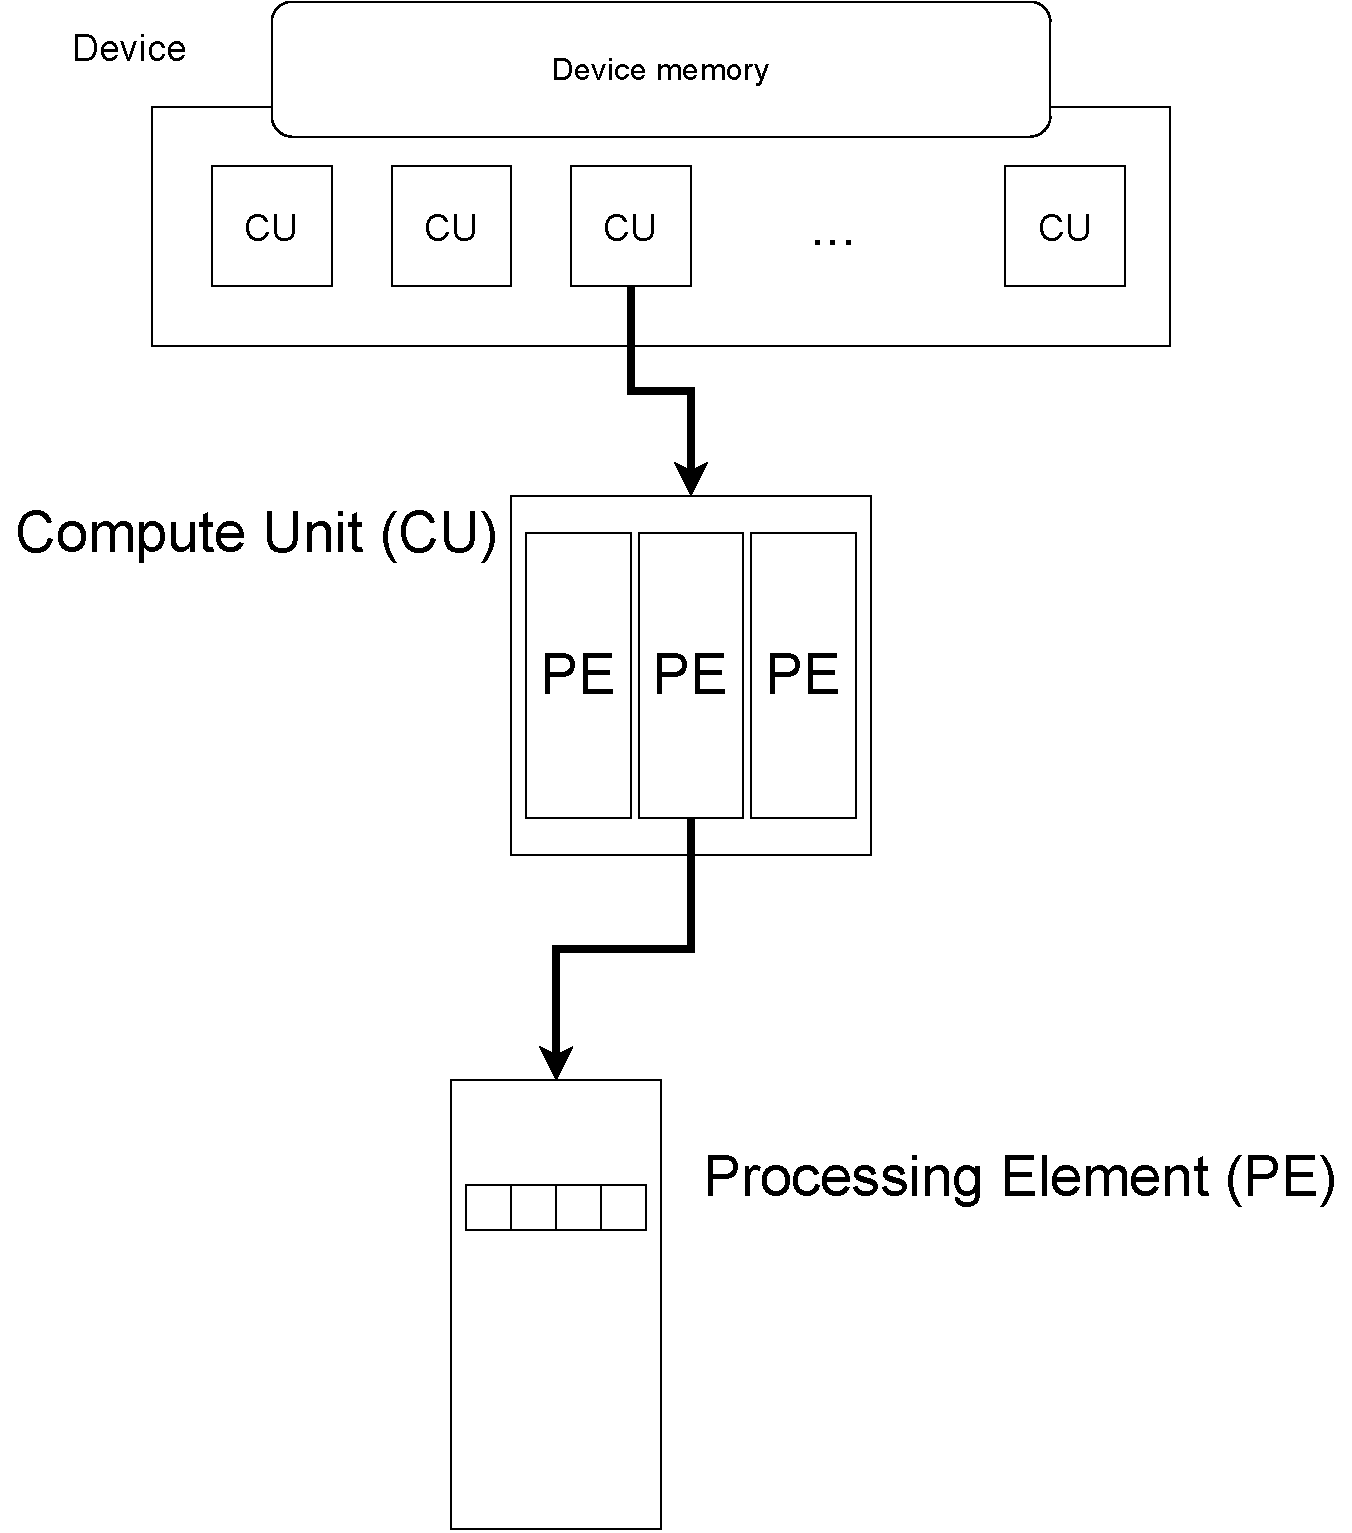
\includegraphics[width=200pt]{\ArtDir/target_device.pdf}}
\caption{A target device is formed of a number of Compute Units (CU). Each of these Compute Units is formed of a number of Processing Elements (PE), which may be able to execute vector (SIMD) instructions.}
\label{figure:target_device_hierarchy}
\end{figure}

The device memory is shared and available to all of the hierarchy of hardware.
Each Compute Unit might in addition provide a layer of memory available only to those Processing Elements contained within it.
This we will call (as in OpenCL) the local memory\index{local memory}.
The Processing Elements in each Compute Unit can access this memory, however it is not accessible by Processing Elements outside the Compute Unit.
We will address using this local memory in OpenMP in Section~\ref{sec:team_only_memory}.

This book will show how to program a device like this, such as GPU, using OpenMP.
In later chapters, we include case studies to show the abstract device model and the concepts in OpenMP come together and are applied to real hardware.


\section{Why you need OpenMP: a single code-base for heterogeneous hardware}

%TGM: There is much more to write here.  I just wanted some placeholder ideas for now.
 Heterogeneous hardware is here today and all indications are hardware will
be more heterogeneous in the future.  Software lasts much longer than hardware.   That means
programmers need to write code that will continue to work as the hardware changes.  

The focus is on performance since that is what parallelism is all about.  But we need to also think about 
maintainability, the ability to maintain an application code-base over the long haul.  Hence, programmers
need to write code with an API that covers heterogeneous hardware across vendors.  And that API
must be one that programmers can be confident will continue to evolve as hardware keeps changing.

OpenMP is a prime candidate to be that API.

\section{The structure of this book}

In the following chapters, we will introduce the necessary concepts for programming heterogeneous systems using OpenMP.

In next chapter we complete laying the foundation for our discussion with an introduction to the core ideas behind OpenMP. 
Experienced OpenMP programmers should just skim that chapter.  We provide 
it as a reminder for people who haven't written much OpenMP code while at the
same time, to establish the jargon of OpenMP that the rest of the book depends on.  We close that chapter with
a taste of what you can do when programming your GPU with OpenMP.   In the multi-core world, people think of OpenMP
as finding key loops and putting a parallel loop directive before that loop.  We close the chapter with the analog to parallel for.  
Its something we call BUD, \emph{the Big Ugly Directive} which for many people will do most of what they need to get started
with programming a GPU from OpenMP.

After our two introductory chapters, we dive into the meat of heterogeneity with OpenMP.  
Each chapter will be split into two.
The first part of each chapter will walk through the most commonly used parts required for obtaining 
good performance on target devices; a ``common core'' for OpenMP target if you will.

The second part of the each chapter will go into some specific details less frequently encountered.
These parts form a comprehensive reference for programming target devices using OpenMP.
As such it covers some of the finer details of the specification that are not required in the main.

The first part alone will be sufficient in the majority of cases for learning most of what is required to 
program GPUs and other devices with OpenMP. Readers are welcome to read only the first part of 
each chapter, and come back to the latter parts if or when they need some additional information on the concepts.


\section{Templates for use in formatting the rest of the book.}

Here is how we handle a code fragment embedded in text.
Consider a simple program that adds two vectors, \code{a} and \code{b}.
\begin{verbatim}
      for (i = 0; i < N; i++) { 
         a[i] = a[i] + b[i];
      }
\end{verbatim}  

For longer code fragments, we put the code in a proper figure.  For example, consider figure~\ref{code:vaddSPMD}

\begin{CodeExample}%
{\textbf{SPMD parallel vector add program} -- \small
Create a team of threads and assign one chunk of loop iterations
to each thread.
}%
{code:vaddSPMD}
\begin{lstlisting}
// OpenMP parallel region and SPMD pattern
#pragma omp parallel
{
   int id, i, Nthrds, istart, iend;
   id = omp_get_thread_num();
   Nthrds = omp_get_num_threads(); 
   istart = id * N / Nthrds;
   iend = (id + 1) * N / Nthrds;
   if (id == Nthrds - 1) iend = N; 
   for (i = istart; i < iend; i++) {
      a[i] = a[i] + b[i];
   }
}
\end{lstlisting}
\end{CodeExample} 



When we have specific constructs to introduce, we use a table with marcros for the constructs themselves.  This way we can make 
sure that we use consistent fonts and styles across the entire book.  Take a look at table~\ref{tab:omp_for} for a good example.

\begin{table}[!htbp]
\centering
\caption{\textbf{A basic worksharing-loop construct in C/C++ and Fortran} 
-- \small
The worksharing-loop construct shares the iterations of a loop among
a team of threads.  The loop is called \texttt{for} in C and \texttt{DO} in Fortran.
Fortran is not block structured, so we need an \texttt{END DO} directive.
Optional clauses give the programmer more control
over the loop construct and include \texttt{schedule}, \texttt{reduction}, and 
\texttt{nowait}. We will discuss these clauses later in this chapter.  Additional clauses define storage attributes 
of the variables used in the worksharing-loop.  We will cover those in 
Chapter~\ref{ch:dataEnv}.  
}
\label{tab:omp_for}
\begin{tabular}{|l|} \hline
\ompbcfor \ompclauses \\ 
%\hspace{5mm} \{   \\
\hspace{5mm} for-loop \\      
%\hspace{5mm} \}    \\           
\hline
\ompbfdo \ompclauses  \\ 
%\hspace{5mm} \{   \\
\hspace{5mm} do-loop   \\
%\hspace{5mm} \}   \\ 
\ompbfdoend \textit{ [nowait] } \\   
                  
\hline

\end{tabular}
\end{table}

Here is an index entry:  Moore's law\index{Moore's law} and a citation Dennard scaling\index{Dennard scaling}~\cite{Dennard}, 


There are some open questions concerning what we need to cover.
\begin{itemize}
\item Do we need to include \code{declare simd}?  Is that enabled for a GPU?  
\item Do we need to discuss the variant directives?  If they are 
important for GPU programmers, then we probably need to. Likewise for assumes and assume.  
\item Does the scan directive apply to GPUs?  
\item Does tile and unroll apply to GPUs?  
\item Do memory spaces apply to GPUs?
\end{itemize}

We will also need to cover a set of internal control variables and where appropriate a set of environment variables.

\begin{table}[h!]
\centering
\caption{All the pragmas we will cover in the book and the chapters where we will cover them}
\label{YourLabel}
%%%%%%%%%%%%%%%%%%%%%%%%%%%%%%%%%%%%%%
%%  
%% The table contains OpenMP pragmas we'll cover in the book
%%
%% To use this in one of our chapters, use the latex command
%%         \begin{table}[h!]
%%          \centering
%%          \caption{Your caption}
%%           \label{YourLabel}
%%           \input{\SubDir/CommonCoreTab.tex}
%%           \end{table}
%%
%%  where the macro \SubDir is defined at the top of each chapter and 
%%  specifies where the source for the book resides.   
%%
%%%%%%%%%%%%%%%%%%%%%%%%%%%%%%%%%%%%%%

\begin{tabular}{|l|l|l|l|}
\hline
\textbf{OpenMP pragma}  & \textbf{Concepts} & \textbf{Chapter} & \textbf{Structure} \\
\hline
%============================================================
\Code{#pragma omp target}                & offload onto a device  & \S\ref{chapter:target} & Core \\ 
\hline 
\Code{#pragma omp teams}                & Create a league of teams & \S\ref{sec:teams} & Core \\
\hline
\Code{#pragma omp distribute}            & Map loops onto a league & \S\ref{ssec:teams_distribute} & Advanced (on its own, favor combined) \\
\hline
\Code{#pragma omp target data}            & Create a device data region & \S\ref{ssec:target_data} & Core \\
\hline
\Code{#pragma omp target enter data}  & Enter a device data region & \S\ref{ssec:target_enter_exit_data} & Core \\
\hline
\Code{#pragma omp target exit data}  & Exit a device data region & \S\ref{ssec:target_enter_exit_data} & Core \\
\hline
\Code{#pragma omp target update}  & Update data between host/device & \S\ref{ssec:target_update} & Core \\
\hline
\Code{#pragma omp loop}  & Concurrent loop iterations & \S\ref{sec:loop} & Core \\
\hline
\Code{#pragma omp requires} & OMP features required & \S\ref{sec:usm} & Core/Advanced \\
\hline
\Code{#pragma omp declare target} & declares items are mapped to a device & \S\ref{ssec:declare_target} & Advanced \\
\hline
\Code{#pragma declare mapper} & user defined mapers & \S\ref{sec:mapper} & Advanced \\
\hline
\Code{#pragma omp interop} & Interoperability with foreign contexts & \S\ref{sec:interop} & Advanced \\
\hline
\Code{teams loop}    & combined construct & \S\ref{sec:loop} & Core \\
\hline
\Code{teams distribute}  & combined  construct & \S\ref{ssec:teams_distribute} & Core \\
\hline
\Code{teams distribute simd}  & combined  construct & XX & Advanced (not useful?) \\
\hline
\Code{teams distribute parallel for} & combined  construct & XX & Advanced \\
\hline
\Code{teams distribute parallel for simd} & combined  construct & \S\ref{sec:bud} & Core \\
\hline
\Code{target parallel}    & combined construct & XX & Advanced \\
\hline
\Code{target simd}    & combined construct & XX & Advanced \\
\hline
\Code{target parallel for}    & combined construct & XX & Advanced \\
\hline
\Code{target parallel for simd}    & combined construct & XX & Advanced \\
\hline
\Code{target parallel loop}    & combined construct & XX & Advanced (N/A?) \\
\hline
\Code{target teams }    & combined construct & XX & Advanced \\
\hline
\Code{target teams loop}    & combined  construct & \S\ref{sec:loop} & Core \\
\hline
\Code{target teams distribute}  & combined  construct & XX & Advanced \\
\hline
\Code{target teams distribute simd}  & combined  construct & XX & Advanced (N/A?) \\
\hline
\Code{target teams distribute parallel for} & combined  construct & XX & Advanced \\
\hline
\Code{target teams distribute parallel for simd} & combined  construct & \S\ref{sec:bud} & Core \\
\hline
\end{tabular}

Comment: best practice often favors the combined constructs (distribute must be strictly nested).

Comment: often the combined construct falls out naturally from explaining what the bits mean.



 \end{table}

\begin{table}[h!]
\centering
\caption{All the clauses we will cover in the book and the chapters where we will cover them}
\label{YourLabel}
%%%%%%%%%%%%%%%%%%%%%%%%%%%%%%%%%%%%%%
%%  
%% The table contains every single clause we will cover from specification
%%
%% To use this in one of our chapters, use the latex command
%%         \begin{table}[h!]
%%          \centering
%%          \caption{Your caption}
%%           \label{YourLabel}
%%           \input{\SubDir/CommonCoreTab.tex}
%%           \end{table}
%%
%%  where the macro \SubDir is defined at the top of each chapter and 
%%  specifies where the source for the book resides.   
%%
%%%%%%%%%%%%%%%%%%%%%%%%%%%%%%%%%%%%%%

\begin{tabular}{|l|l|l|l|}
\hline
\textbf{OpenMP clauses}  & \textbf{Constructs} & \textbf{Chapter} & \textbf{Structure} \\
\hline
%============================================================
\Code{private}                   & teams, distribute, simd, loop, target & \S\ref{sssec:data_sharing} & Core \\
\hline
\Code{firstprivate}              & teams & \S\ref{sssec:data_sharing} & Core \\
\hline
\Code{lastprivate}              & distribute, simd, loop   & \S\ref{sssec:data_sharing} & Advanced \\
\hline
\Code{shared}           & teams & \S\ref{sssec:data_sharing} & Core (concept) / Advanced (clause itself)\\
\hline
\Code{reduction}           & teams, parallel & \S\ref{sec:reduction} and \S\ref{sec:target_reductions} & Core \\
\hline
\Code{allocate}           & (allocator for private variables) target, teams, distribute & XX & Advanced (N/A?) \\
\hline
\Code{default}           & teams & XX & Advanced \\
\hline
\Code{num_teams}           & teams & \S\ref{ssec:gpu_specific_mapping} & Advanced \\
\hline
\Code{thread_limit}           & target, teams & XX & Advanced (N/A?) \\
\hline
\Code{reduction}    & simd, loop & see above & Core \\
\hline
\Code{in\_reduction}    & target & \S\ref{sec:in_reduction} & Advanced \\
\hline
\Code{collapse}      & simd, loop & \S\ref{ssec:fork_join} & Core \\
\hline
\Code{dist\_schedule}    & distribute & \S\ref{ssec:teams_distribute} & Core (but not recommended) \\
\hline
\Code{order}                   & distribute, loop & XX & Advanced \\
\hline
\Code{bind}              & loop & XX & Advanced (esoteric) \\
\hline
\Code{if}            & simd, target, target data, target enter data, target exit data & \S\ref{sec:if_clause} & Advanced (might be Core?)\\
\hline
\Code{safelen}   & simd & XX & N/A \\
\hline
\Code{simdlen}   & simd & XX & Advanced? (N/A) \\
\hline
\Code{aligned}   & simd & XX & N/A \\
\hline
\Code{linear}      & simd & XX & N/A \\
\hline
\Code{nontemporal}   & simd & XX & N/A \\
\hline
\Code{map}      & target, target data, target enter data, target exit data, declare mapper & \S\ref{ssec:map_clause} & Core \\
\hline
\Code{use\_device\_ptr}    & target data (interop) & XX & Advanced \\
\hline
\Code{is\_device\_ptr}    & target (interop, alloc APIs) & \S\ref{sec:alloc_apis} & Advanced \\
\hline
\Code{use\_device\_addr}     & target data (interop) & XX & Advanced \\
\hline
\Code{has\_device\_addr}     & target (interop, alloc APIs) & \S\ref{sec:alloc_apis} & Advanced \\
\hline
\Code{uses\_allocaters}    & target data & XX & Advanced (esoteric) \\
\hline
\Code{device}           & target,target data, target enter data, target exit data, interop & \S\ref{sec:host_device_model} and multi-gpu section & Core \\
\hline
\Code{depend}      & target,target enter data, target exit data, interop & \S\ref{chapter:async} & Core \\
\hline
\Code{nowait}     & target,target enter data, target exit data, interop & \S\ref{chapter:async} & Core \\
\hline
\Code{to/from}    & update & \S\ref{ssec:target_update} & Core \\
\hline
\Code{to}    & declare\_target & \S\ref{ssec:declare_target} & Advanced \\
\hline
\Code{link}    & declare\_target & \S\ref{ssec:declare_target} & Advanced \\
\hline
\Code{device\_type}   & declare\_target & \S\ref{ssec:declare_target} & Advanced \\
\hline
\Code{indirect}     & declare\_target & \S\ref{ssec:declare_target} & Advanced \\
\hline
\Code{init}      & interop & XX & Advanced \\
\hline
\Code{destroy}   & interop & XX & Advanced \\
\hline
\Code{use}       & interop & XX & Advanced \\
\hline
\end{tabular}

Comment: simd clauses same as from Next Steps book.






 \end{table}
 
\begin{table}[h!]
\centering
\caption{All the runtime functions we will cover in the book and the chapters where we will cover them}
\label{YourLabel}
%%%%%%%%%%%%%%%%%%%%%%%%%%%%%%%%%%%%%%
%%  
%% The table contains every single runtime function we will cover from specification
%%
%% To use this in one of our chapters, use the latex command
%%         \begin{table}[h!]
%%          \centering
%%          \caption{Your caption}
%%           \label{YourLabel}
%%           \input{\SubDir/CommonCoreTab.tex}
%%           \end{table}
%%
%%  where the macro \SubDir is defined at the top of each chapter and 
%%  specifies where the source for the book resides.   
%%
%%%%%%%%%%%%%%%%%%%%%%%%%%%%%%%%%%%%%%

\begin{tabular}{|l|l|}
\hline
\textbf{OpenMP functions,}  & Chapter \\
\hline
%============================================================
\Code{int omp\_get\_team\_size()}      & XX \\
\hline
\Code{int omp\_get\_num\_teams()}       & XX   \\
\hline
\Code{int omp\_get\_team\_num()}       & XX   \\
\hline
\Code{void omp\_set\_num\_teams()}       & XX    \\
\hline
\Code{int omp\_get\_max\_teams()}      & XX    \\
\hline
\Code{void omp\_set\_teams\_thread\_limit()}     & XX    \\
\hline
\Code{int omp\_get\_teams\_thread\_limit()}      & XX    \\
\hline
\Code{int omp\_get\_teams\_thread\_limit()}      & XX    \\
\hline
\Code{int omp\_pause\_resource()}      & XX    \\
\hline
\Code{int omp\_pause\_resource\_all()}    & XX    \\
\hline
\Code{int omp\_get\_num\_procs()}     & XX    \\
\hline
\Code{void omp\_set\_default\_device()}    & XX    \\
\hline
\Code{int omp\_get\_default\_device()}          & XX    \\
\hline
\Code{int omp\_get\_num\_devices()}         & XX    \\
\hline
\Code{int omp\_get\_device\_num()}       & XX    \\
\hline
\Code{int omp\_is\_initial\_device()}         & XX    \\
\hline
\Code{int omp\_get\_initial\_device()}          & XX    \\
\hline
\Code{void* omp\_target\_alloc()}        & XX    \\
\hline
\Code{void omp\_target\_free()}        & XX    \\
\hline
\Code{int omp\_target\_is\_present()}           & XX    \\
\hline
\Code{int omp\_target\_is\_axxessible()}          & XX    \\
\hline
\Code{int omp\_target\_memcpy()}          & XX    \\
\hline
\Code{int omp\_target\_memcpy_rect()}          & XX    \\
\hline
\Code{int omp_target_memcpy_async()}          & XX    \\
\hline
\Code{int omp_target_memcpy_rect_async()}          & XX    \\
\hline
\Code{int omp_target_associate_ptr()}          & XX    \\
\hline
\Code{omp_target_disassociate_ptr()}          & XX    \\
\hline
\Code{void *omp_get_mapped_ptr()}          & XX    \\
\hline
\Code{int omp_get_num_interop_properties()}          & XX    \\
\hline
\Code{int omp_get_num_interop_properties()}          & XX    \\
\hline
\Code{void *omp_get_interop_ptr()}          & XX    \\
\hline
\Code{void *omp_get_interop_ptr()}          & XX    \\
\hline
\Code{const char* omp_get_interop_name()}          & XX    \\
\hline
\Code{const char* omp_get_interop_type_desc()}          & XX    \\
\hline
\Code{const char* omp_get_interop_rc_desc ()}          & XX    \\
\hline
\end{tabular}




 \end{table}
 
\begin{table}[h!]
\centering
\caption{All the internal control variables and associated environment variables we will 
cover in the book and the chapters where we will cover them}
\label{YourLabel}
%%%%%%%%%%%%%%%%%%%%%%%%%%%%%%%%%%%%%%
%%  
%% The table contains OpenMP ICVs and Env Vars we'll cover in the book
%%
%% To use this in one of our chapters, use the latex command
%%         \begin{table}[h!]
%%          \centering
%%          \caption{Your caption}
%%           \label{YourLabel}
%%           \input{\SubDir/CommonCoreTab.tex}
%%           \end{table}
%%
%%  where the macro \SubDir is defined at the top of each chapter and 
%%  specifies where the source for the book resides.   
%%
%%%%%%%%%%%%%%%%%%%%%%%%%%%%%%%%%%%%%%

\begin{tabular}{|l|l|l|}
\hline
\textbf{ICV}  & Env var & Chapter \\
\hline
%============================================================
\Code{thread-limit-var}                & \Code{OMP\_THREAD\_LIMIT} & XX \\ 
\hline 
\Code{default-device-var}                & \Code{OMP\_DEFAULT\_DEVICE} & XX \\
\hline
\Code{target-offload-var}            & \Code{OMP\_TARGET\_OFFLOAD} & XX \\
\hline
\Code{nteams-var}            & \Code{OMP\_NUM\_TEAMS} & XX \\
\hline
\Code{teams-thread-limit-var}  & \Code{OMP\_TEAMS\_THREAD\_LIMIT} & XX \\
\hline
\end{tabular}



 \end{table}


%-----------------------------------------------------------------------
%------------------------- From Next Step ------------------------------
%-----------------------------------------------------------------------
%\section{From The Next Step Chapter 6}
%
%Specialized accelerator processors, which dramatically improve the performance
%of some computations, are proliferating, and general-purpose processors are
%now very often connected to some type of accelerator.  
%The popularity of these heterogeneous architectures across all types of
%computing has had a noticeable impact on the development of software.  
%
%To exploit these systems, developers must write software that executes various
%regions of code on different types of devices.  There are many reasons for
%wanting to do this but very often the motivation is to accelerate
%computationally intensive loop nests.  
%
%However, the programming models for these systems are difficult to use.
%Often code modules are written twice, once for the general-purpose
%processor and then again for the accelerator.  The accelerator version is often
%written in a lower-level, accelerator-specific language.  The result is the
%undesirable software maintenance problem of keeping two versions of code, which
i%mplement the same algorithm, synchronized.

%The \OMP\ Language Committee recognized the need to make it easier to program
%heterogeneous architectures and set about to extend \OMP\ to support these types
%of systems \cite{Beyer2011}.  The results of this work were initially released
%in \OMPfourzero\ and updated in \OMPfourfive.
%
%Software developers can use \OMP\ to program accelerators in a higher-level
l%anguage and maintain one version of their code, which can run on either an
%accelerator or a general-purpose processor.  In this chapter, we present the
%syntax for and describe how to use the \OMP\ \emph{device constructs} and
%related runtime functions that were added to support heterogeneous
%architectures. 

%What was needed is a programming model that could...
%Given the popularity of heterogeneous systems across all types of computing,

%There is a place here for \OMP\ to make these software packages more
%maintainable and portable.  We hope that in the future, as the latest versions
%of \OMP\ are implemented in more compilers, software developers will leverage
%the \OMP\ device constructs and develop one version of their code that can run
%anywhere, including on accelerators.

%There is a place here for \OMP\ to make these software packages more
%maintainable and portable.  We hope that in the future, as the latest versions
%of \OMP\ are implemented in more compilers, 
